% CU CS5525
% Fall 2012
% Python Compiler
%
% slides.tex
% Semester Project Slides
%
% Repository:
%    https://github.com/asayler/CU-CS5525-PythonCompiler
%
% By :
%    Anne Gatchell
%       http://annegatchell.com/
%    Andy Sayler
%       http://www.andysayler.com
%    Michael (Mike) Vitousek
%       http://csel.cs.colorado.edu/~mivi2269/

\documentclass{beamer}
\usetheme{Montpellier}
\usecolortheme{beaver}
%\setbeamercovered{transparent=25}
\setbeamertemplate{blocks}[rounded][shadow=false]
\setbeamertemplate{navigation symbols}{}
\setcounter{tocdepth}{1}

\usepackage{graphicx}
\usepackage{url}
\usepackage{listings}
\usepackage{biblatex}
\usepackage{amssymb}
\bibliography{refs}

\hypersetup{
    colorlinks,
    citecolor=black,
    filecolor=black,
    linkcolor=black,
    urlcolor=black
}

\lstset{
  language={},
  basicstyle=\footnotesize,
  numbers=none,
  numberstyle=\tiny,
  stepnumber=1,
  numbersep=5pt,
  showspaces=false,
  showstringspaces=false,
  showtabs=false,
  tabsize=4,
  captionpos=b,
  breaklines=true,
  breakatwhitespace=false,
  frame=single,
  frameround=tttt
}

\lstdefinelanguage{llvm}{
  morecomment = [l]{;},
  morestring=[b]'', 
  sensitive = true,
  classoffset=0,
  morekeywords={
    define, declare, global, constant,
    internal, external, private,
    linkonce, linkonce_odr, weak, weak_odr, appending,
    common, extern_weak,
    thread_local, dllimport, dllexport,
    hidden, protected, default,
    except, deplibs,
    volatile, fastcc, coldcc, cc, ccc,
    x86_stdcallcc, x86_fastcallcc,
    ptx_kernel, ptx_device,
    signext, zeroext, inreg, sret, nounwind, noreturn,
    nocapture, byval, nest, readnone, readonly, noalias, uwtable,
    inlinehint, noinline, alwaysinline, optsize, ssp, sspreq,
    noredzone, noimplicitfloat, naked, alignstack,
    module, asm, align, tail, to,
    addrspace, section, alias, sideeffect, c, gc,
    target, datalayout, triple,
    blockaddress
  },
  classoffset=1,
  morekeywords={
    fadd, sub, fsub, mul, fmul,
    sdiv, udiv, fdiv, srem, urem, frem,
    and, or, xor,
    icmp, fcmp,
    eq, ne, ugt, uge, ult, ule, sgt, sge, slt, sle,
    oeq, ogt, oge, olt, ole, one, ord, ueq, ugt, uge,
    ult, ule, une, uno,
    nuw, nsw, exact, inbounds,
    phi, call, select, shl, lshr, ashr, va_arg,
    trunc, zext, sext,
    fptrunc, fpext, fptoui, fptosi, uitofp, sitofp,
    ptrtoint, inttoptr, bitcast,
    ret, br, indirectbr, switch, invoke, unwind, unreachable,
    malloc, alloca, free, load, store, getelementptr,
    extractelement, insertelement, shufflevector,
    extractvalue, insertvalue,
  },
  alsoletter={\%},
  keywordsprefix={\%},
}

\newenvironment{packed_enum}{
\begin{enumerate}
  \setlength{\itemsep}{1pt}
  \setlength{\parskip}{0pt}
  \setlength{\parsep}{0pt}
}{\end{enumerate}}

\newenvironment{packed_item}{
\begin{itemize}
  \setlength{\itemsep}{1pt}
  \setlength{\parskip}{0pt}
  \setlength{\parsep}{0pt}
}{\end{itemize}}

\title[LLVM Compiler]{
  Building a LLVM Python Compiler
}

\author[Gatchell, Sayler, Vitousek]{
  Anne Gatchell    \and
  Andy Sayler      \and
  Michael Vitousek
}

\institute[CU Boulder]{
  University of Colorado at Boulder   \\
  \texttt{anne.gatchell@colorado.edu} \\
  \texttt{andrew.sayler@colorado.edu} \\
  \texttt{michael.vitousek@colorado.edu}
}

\date{\today}

\begin{document}

%---Title Slide---%
\begin{frame}[plain]
  \titlepage
\end{frame}

%---TOC Slide---%
\begin{frame}{Outline}
  \tableofcontents
\end{frame}

\section{Introduction}

%---Goals Slide---%
% Anne
\begin{frame}{\bf Goals}
  \begin{itemize}
  \item<1-> Create Low Level Virtual Machine (LLVM) p3-compliant compiler
    \begin{itemize}
    \item<1-> Make our compiler multi-platform
    \item<1-> Explore LLVM architecture
    \item<1-> Learn LLVM standard
    \end{itemize}
  \item<2-> Compare to x86 compiler
  \item<3-> Test on multiple architectures(x86, ARM, etc.)
  \end{itemize}
\end{frame}

\section{Background}

\subsection{LLVM}

%---Background Slide---%
% Andy
\begin{frame}{\bf LLVM Basics}
  \begin{itemize}
  \item<1->Open Source
  \item<2->Static Single Assembly (SSA)
  \item<3->Multi-platform support (x32, x64, ARM, etc)
  \item<4->Multi-runtime support (compiled, interpreted, JIT, etc.)
  \item<5->Becoming a very popular compiler infrastructure and IR
    \begin{itemize}
    \item<5-> Used heavily in OSX and IOS systems
    \item<5-> Targeted to replace legacy GCC implementation (clang,
      gcc-llvm, etc)
    \item<5-> Used in heterogeneous platforms (CPU + GPU, etc) to
      dynamically target code at different processors
    \end{itemize}
  \end{itemize}
\end{frame}

%---LLVM Background Slide---%
% Andy
\begin{frame}{\bf LLVM Concepts}
  \begin{itemize}
  \item<1->LLVM Intermediate Representation (IR)
    \begin{itemize}
    \item<2->In-memory data structure
    \item<3->Human readable ``assembly'' language (.ll)
    \item<4->File-oriented bitcode (colloqially, bytecode) (.bc)
    \end{itemize}
  \item<5->We convert to assembly (.ll) code
  \item<6->Example...
  \end{itemize}
\end{frame}

%---LLVM Hello World Slide---%
% Andy
\begin{frame}{\bf LLVM ``Hello World''}
  \lstinputlisting[
    language=llvm,
    title={LLVM Assembly - Hello World Example \cite{lattner-llvmlangref}}
  ]{../code/llvm-examples/hello0.ll}
\end{frame}

\section{Design}

\subsection{Design Overview}

%---Project Approach Slide---%
% Anne
\begin{frame}{Approach}
  \begin{itemize}
  \item<1->Refactored existing compiler to fix all known issues, add
    features, etc.
  \item<2->"Compiled" tests programs by hand to LLVM IR for reference
  \item<3->Added an SSA Conversion pass after Flatten pass
  \item<4->Added an LLVM Instruction Selection pass to produce LLVM IR
  \item<5->Modified build and test system to handle both x86 and LLVM
  \item<6->Tested and compared Python, x86, and LLVM execution
  \end{itemize}
\end{frame}

\subsection{Module Flow}

%---Module Flow Slide---%
% Anne
\begin{frame}{\bf Module Flow}
  \begin{center}
    \includegraphics[height=.75\paperheight]{./include/CompilerFlow.pdf}
  \end{center}
\end{frame}


\subsection{SSA Conversion}

%---SSA Overview---%
% Mike
\begin{frame}{Static Single Assignment Form}
  \begin{itemize}
  \item<1->Each variable assigned only once
  \item<2->If branching involved, use phi nodes
  \item<3->LLVM has phi node already integrated
  \end{itemize}
\end{frame}

%---Simple SSA Conversion---%
% Mike
\begin{frame}{\bf Simple conversion}
  \lstinputlisting[
  language=python,
  label=lst:ssa-step1,
]{include/py/ssa-step1.py}
\pause
  \lstinputlisting[
  language=python,
  label=lst:ssa-step2,
]{include/py/ssa-step2.py}
\end{frame}

%---If SSA Conversion---%
% Mike
\begin{frame}[shrink]{\bf SSA Conversions of If statements}
  \lstinputlisting[
  language=python,
  label=lst:ssa-if1,
]{include/py/ssa-if1.py}
\pause
  \lstinputlisting[
  language=python,
  label=lst:ssa-if2,
]{include/py/ssa-if2.py}
\end{frame}

%---While SSA Conversion---%
% Mike
\begin{frame}[shrink]{\bf SSA Conversions of While statements}
  \lstinputlisting[
  language=python,
  label=lst:ssa-while1,
]{include/py/ssa-while1.py}
\pause
  \lstinputlisting[
  language=python,
  label=lst:ssa-while2,
]{include/py/ssa-while2.py}
\end{frame}

\subsection{Instruction Selection}

%---Instruction Selection overview---%
% Andy
\begin{frame}{LLVM Features and Restrictions}
  LLVM is higher level than x86. This means...
  \pause
  \begin{itemize}
  \item<1->It has more features
    \begin{itemize}
    \item<2->Unlimited registers
    \item<3->Powerful and generalized functions (switch, compare, etc)
    \item<4->Built-in stack and function management
    \end{itemize}
  \item<5->But also more restrictions
    \begin{itemize}
      \item<6-> No loose casting: types are enforced
      \item<7-> External functions must be declared
      \item<8-> Direct assignments (x=5, a=b) not allowed
    \end{itemize}
  \end{itemize}
\end{frame}


%---Instruction Selection Blocks---%
% Andy
\begin{frame}{LLVM Blocks}
  To be added...
\end{frame}

\begin{frame}{Pyobjs to Handle Polymorphism}
\begin{itemize}
  \item<1->LLVM is typed
  \item<2->Pointers to Pyobjs give us freedom
  \item<3->Except in indirect function calls
\end{itemize}
\end{frame}

%---Indirect Function Calls---%
% Anne
\begin{frame}{\bf Indirect Function Calls}
  \lstinputlisting[
    language=llvm,
    title={LLVM Assembly - Dealing with Lambdas}
  ]{include/ll/llvm_func_ptr.ll}
\end{frame}

%---Strings---%
% Anne
\begin{frame}[shrink]{\bf Strings}
  \begin{itemize}
  \item<1->Strings defined much like x86
  \item<2->Type is an array
  \item<3->Call getelementptr to get the string by accessing array
  \end{itemize}
  \pause
  \lstinputlisting[
    language=llvm,
    label=lst:LLVM Assembly - Dealing with Strings,
  ]{include/ll/strings.ll}
\end{frame}

\subsection{LLVM Build Process}

%---Build Process---%
% Anne
\begin{frame}{LLVM Build Chain}
\begin{itemize}
  \item<1->LLVM assembler (llvm-as) to bitcode (.bc)
  \item<2->Use Clang and llvm-as to get bitcode of runtime files
  \begin{itemize}
    \item<2->clang -emit-llvm -S helper/runtime.c -o build/runtime.ll
    \item<2->llvm-as  build/runtime.ll -o build/runtime.bc
  \end{itemize}
  \item<3->Link (llvm-link) all files
  \item<4->LLVM compiler (llc) OR LLVM interpreter (lli)
  \item<5->Use gcc or clang to compile to code for machine 
  \begin{itemize}
    \item<5->eg. clang -g -x assembler build/test-p0-1.lls -lm -o build/test-p0-1.llout
  \end{itemize}
  \end{itemize}
\end{frame}

\section{Results}

%---Benchmark Results---%
% Mike
\begin{frame}{Benchmark Results}
  \begin{center}
    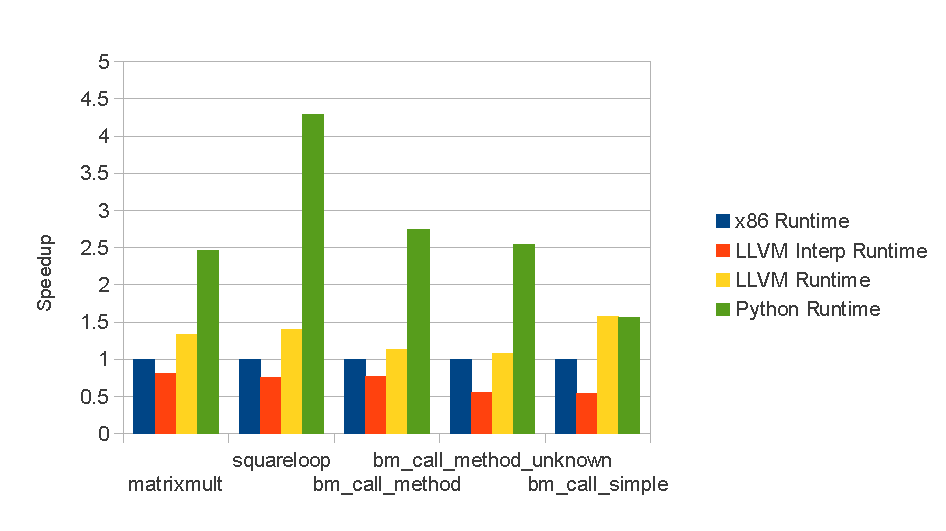
\includegraphics[scale=.63]{./include/pdf/runtime.pdf}
  \end{center}
  \begin{itemize}
  \item $10\%$ to $60\%$ speedup at runtime
  \end{itemize}
\end{frame}

\begin{frame}{Benchmark Results}
  \begin{center}
    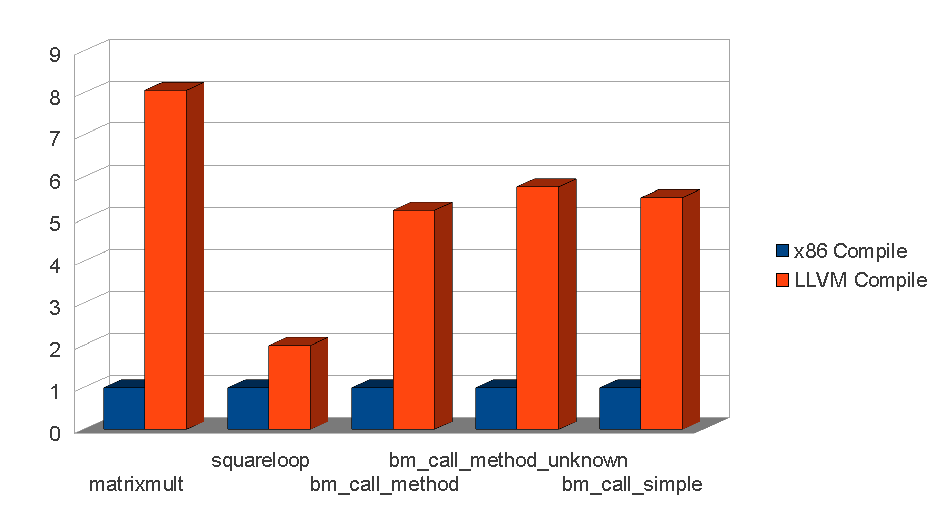
\includegraphics[scale=.63]{./include/pdf/compiletime.pdf}
  \end{center}
  \begin{itemize}
  \item $2$x to $6$x compile time speedup\pause, due to register allocation
  \end{itemize}
\end{frame}

\section{Demo}

%---Live Demo---%
% Andy
\begin{frame}{Demo}
  A Demo...
\end{frame}

%---Bibliography Slide---%
\begin{frame}[t,allowframebreaks]{\bf Bibliography}
  \nocite{*}
  \printbibliography
\end{frame}

\end{document}
